\documentclass[9pt]{beamer}

\usetheme[progressbar=frametitle,block=fill,background=light]{metropolis}
\usefonttheme{serif}

\usepackage{appendixnumberbeamer}

\usepackage{booktabs}
\usepackage[scale=2]{ccicons}


\usepackage{pgfplots}
\usepgfplotslibrary{dateplot}
\usepackage{pgfplotsthemetol}
\usepackage{amsmath,amssymb,amsthm,amsfonts,amstext}
\usepackage{bbm}
\usepackage{array}
\usepackage{multimedia}
\usepackage{media9}
\usepackage{caption}
\usepackage{subcaption}

\usepackage{xspace}

\usepackage{import}
\import{}{Packages/custom_macros.tex}

\makeatletter
\setlength{\metropolis@titleseparator@linewidth}{2pt}
\setlength{\metropolis@progressonsectionpage@linewidth}{2pt}
\setlength{\metropolis@progressinheadfoot@linewidth}{2pt}
\makeatother

\newcommand{\themename}{\textbf{\textsc{metropolis}}\xspace}
\renewcommand{\emph}{\alert}
\newcommand{\pencil}{
\includegraphics[scale=0.07]{Pictures/pen.png}}
\renewcommand{\Re}{\text{Re}}
\renewcommand{\Im}{\text{Im}}

\title{Group theory, Topology and Spin-$1/2$ Particles}
\subtitle{From Dirac's belt to fermions}
% \date{\today}
\date{}
\author{Louan Mol}
\institute{Unversité Libre de Bruxelles\\[2cm]{\small Brussels Summer School of Mathematics 2022}}
% \titlegraphic{\hfill\includegraphics[height=1.5cm]{logo.pdf}}

\begin{document}

\maketitle

\nocite{*}

\begin{frame}{Table of contents}
    \setbeamertemplate{section in toc}[sections numbered]
    \tableofcontents%[hideallsubsections]
\end{frame}

\section{Dirac's belt trick and the rotation group}

\begin{frame}{Dirac's belt trick}
    
    You need:
    \begin{itemize}
        \item a belt (not necessarily Dirac's)
        \item a heavy book
    \end{itemize}

    \textbf{Goal:} deform the belt to untwist a $2\pi$-twist.\\[0.2cm]

    Note: deforming the belt is equivalent to moving its ends and keep the same orientation.\\[0.2cm]
    
    $\Rightarrow$ it tuns out to be \emph{impossible} ! One turn negates the twist: $2\pi\to-2\pi$.\\[0.2cm]

    However, possible for a $4\pi$ twist ...\\ \hspace{7cm} Why is that ?

\end{frame}

%\begin{frame}{Anti-twister mechanisms}
%    \begin{center}
%        \movie[width=4cm,height=2.5cm,showcontrols,loop]{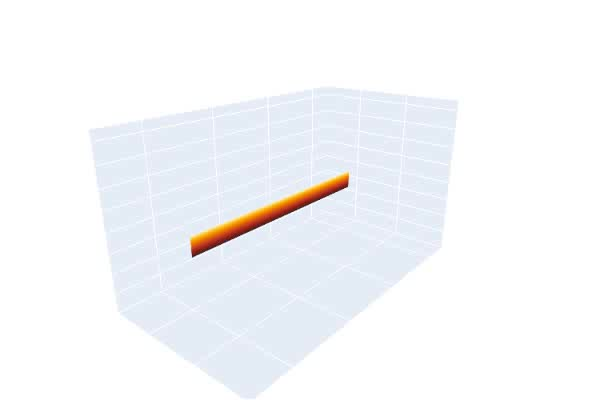
\includegraphics[scale=0.15]{Pictures/poster3.jpg}}{Videos/BeltTrick.wmv}
%    \end{center}
%\end{frame}

\begin{frame}{Space of rotations: $\SO(3)$ as a group}
      
    What is a rotation in $\R^3$ ? It is a real $3\times3$ matrix $R$ that must
    \begin{enumerate}
        \item preserve the \emph{scalar product}: $R^TR=\mathbbm{1}$ ($\Leftrightarrow$ $R$ is orthogonal)
        \item preserve the \emph{orientation}: $\det R=1$
    \end{enumerate}

    \begin{block}{Special othogonal group}
        $\SO(3)$ is the set of $3\times 3$ real matrices such that $R^TR=\mathbbm{1}$ and $\det R=1$.
    \end{block}
    Three ``fundamental'' rotations:
    \begin{equation*}
      {\tiny
      x:
      \begin{bmatrix}
          1 & 0 & 0 \\
          0 & \cos\theta & -\sin\theta \\
          0 & \sin\theta & \cos\theta
      \end{bmatrix}\qquad
      y:
      \begin{bmatrix}
          \cos\theta & 0 & -\sin\theta \\
          0 & 1 & 0 \\
          \sin\theta & 0 & \cos\theta
      \end{bmatrix}\qquad
      z:
      \begin{bmatrix}
          \cos\theta & -\sin\theta & 0 \\
          \sin\theta & \cos\theta & 0 \\
          0 & 0 & 1
      \end{bmatrix}}
    \end{equation*}
    any rotation can be obtained by composing those three rotation.\\[0.2cm]

    $\Rightarrow$ It forms a \emph{group}.
    
\end{frame}

\begin{frame}{Space of rotations: $\SO(3)$ as a manifold}

    Fundamental data that describes a rotation:
    \begin{itemize}
        \item an \emph{axis} of rotation, i.e. a  unit vector $\overrightarrow{n}$ \hspace{1.07cm}\textcolor{blue}{$\to$ 2 parameters}
        \item an \emph{angle} of rotation $\theta\in[-\pi,\pi]$ (with $-\pi\sim\pi$) \textcolor{blue}{$\to$ 1 parameter}
    \end{itemize}
    The space of rotations can then alternately be defined as a \textbf{$\boldsymbol{3}$-sphere of radius $\boldsymbol{\pi}$ and its antipodal points identified}:

    \begin{columns}[T,onlytextwidth]
        \column{0.5\textwidth}

            \vspace{0.5cm}
            \begin{equation*}
              \boxed{\SO(3)\cong B^3(\pi)/\sim}
            \end{equation*}
            and for each point:
            \begin{align*}
                \text{direction} &\leftrightarrow \text{axis}\\
                \text{norm} &\leftrightarrow \text{angle}
            \end{align*}
            $\Rightarrow$ It is also a \emph{manifold} , most \\
            \hspace{0.3cm} famously known as $\R\P^3$.
  
        \column{0.5\textwidth}
  
            \begin{figure}
                \centering
                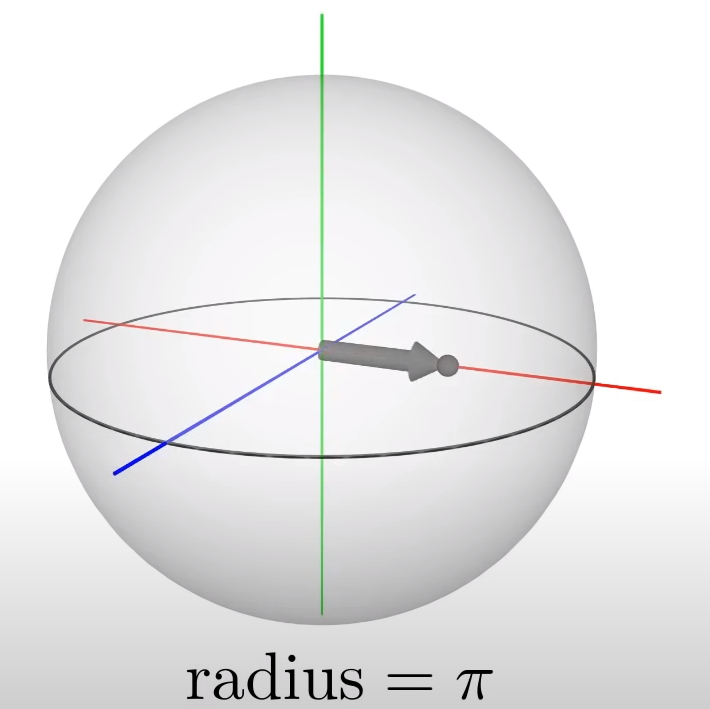
\includegraphics[scale=0.16]{Pictures/SO3sphere.png}
            \end{figure}
  
    \end{columns}

    We have $\dim(\SO(3))=3$.\\[0.2cm]
    (Note that group $+$ manifold $=$ Lie group.)
    
\end{frame}

\begin{frame}{Back to the belt}

    Mathematical description of the belt ?\\[0.3cm]
    \quad $\triangleright$ a belt is a strip, which is just a \emph{path} $+$ an \emph{orientation}.\\[0.2cm]
    \quad $\triangleright$ given axis on the middle line along the belt, each set of axis \\ \hspace{0.5cm} is related by a rotation \\[0.2cm]
    \quad $\triangleright$ a belt configuration is equivalent to a continuous set of axis and \\ \hspace{0.5cm} therefore to a continuous set of translations, i.e. a \emph{path in $\SO(3)$}
    \begin{figure}
        \centering
        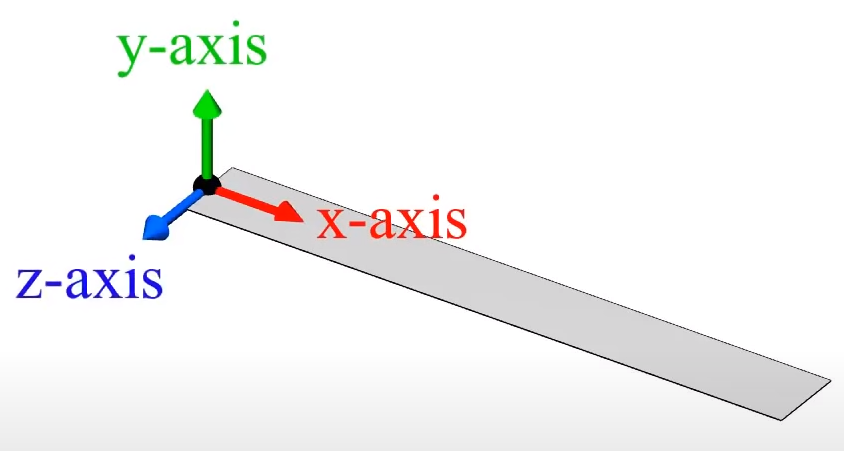
\includegraphics[scale=0.12]{Pictures/beltaxis.png}
    \end{figure}
    There is a bijection:
    \begin{equation*}
        \boxed{\text{belt configuration} \Leftrightarrow \text{path in $\SO(3)$}}
    \end{equation*}
    This gives us a new language to analyze the problem !

\end{frame}

\begin{frame}{Examples}
    \makebox[315pt][r]{
    \begin{tabular}{cccc}
        \textbf{\underline{trivial rotation}} & \textbf{\underline{$2\pi$ \textcolor{red}{$x$}-rotation}} & \textbf{\underline{$2\pi$ \textcolor{green}{$y$}-rotation}} & \textbf{\underline{$2\pi$ \textcolor{blue}{$z$}-rotation}}\\
        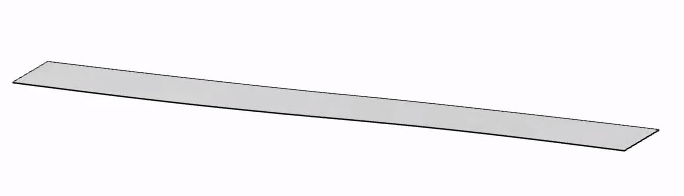
\includegraphics[scale=0.12]{Pictures/flatbelt.png} & 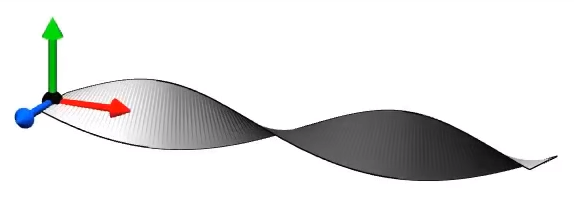
\includegraphics[scale=0.12]{Pictures/xaxisbelt.png} & 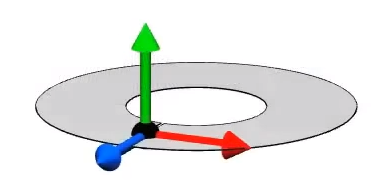
\includegraphics[scale=0.15]{Pictures/yaxisbelt.png} & 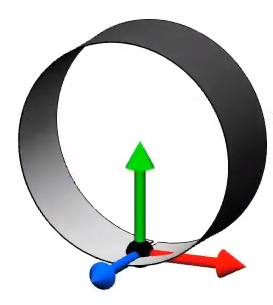
\includegraphics[scale=0.15]{Pictures/zaxisbelt.png} \\
        $\updownarrow$ & $\updownarrow$ & $\updownarrow$ & $\updownarrow$ \\
        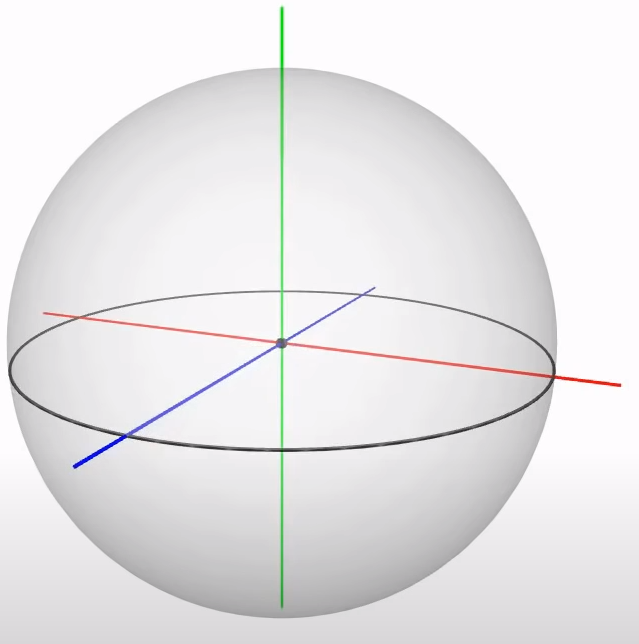
\includegraphics[scale=0.1]{Pictures/4pisphere4.png} & 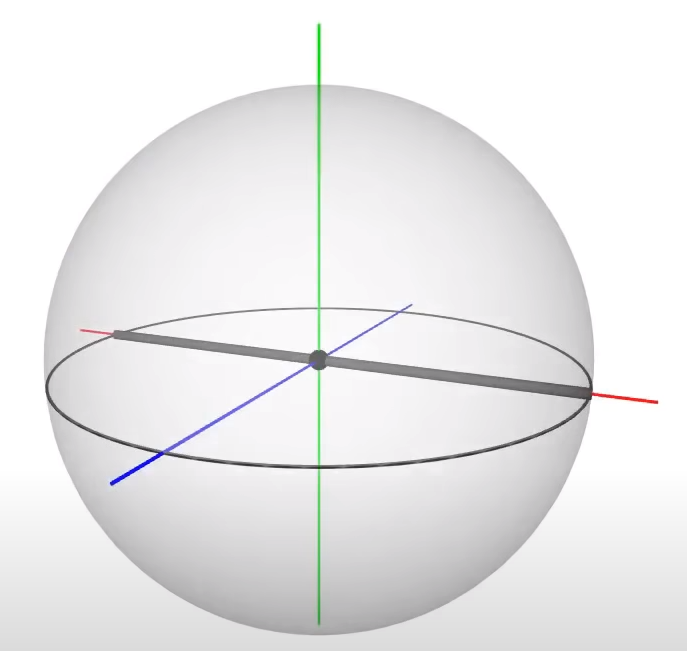
\includegraphics[scale=0.1]{Pictures/xaxissphere.png} & 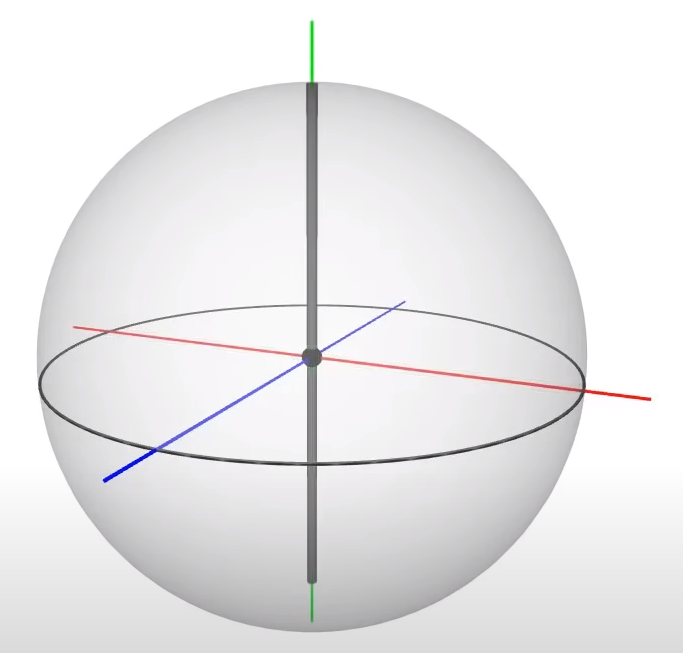
\includegraphics[scale=0.1]{Pictures/yaxissphere.png} & 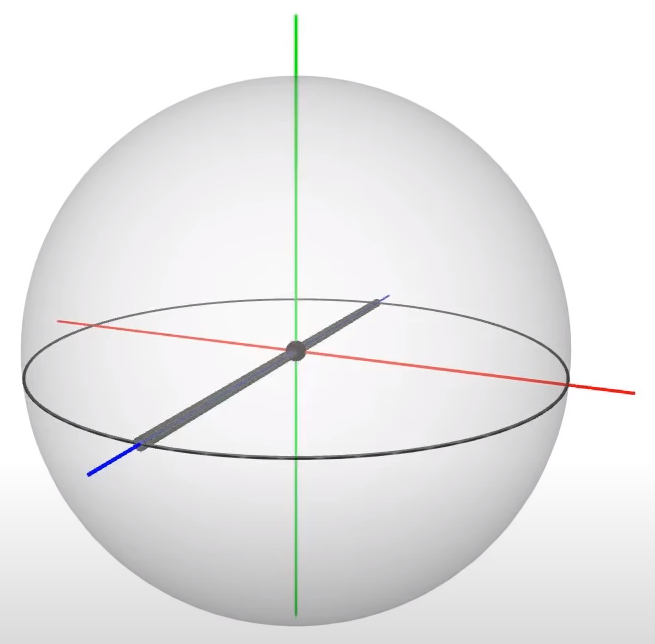
\includegraphics[scale=0.1]{Pictures/zaxissphere.png}
    \end{tabular}}
\end{frame}

\begin{frame}{Examples}
    \begin{center}
    \begin{tabular}{ccc}
        \textbf{\underline{random rotation}} & \textbf{\underline{closed}} & \textbf{\underline{open path}}\\
        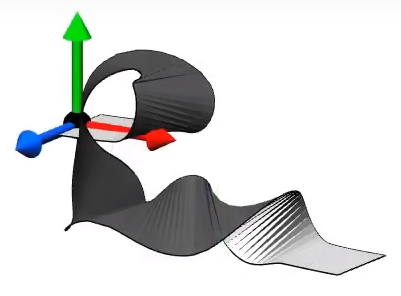
\includegraphics[scale=0.15]{Pictures/randomrotbelt.png} & 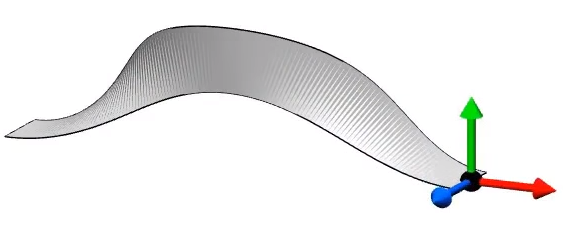
\includegraphics[scale=0.1]{Pictures/contractiblepathbelt.png} & 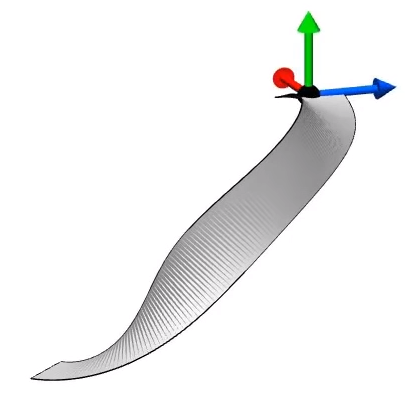
\includegraphics[scale=0.1]{Pictures/noncontractiblepathbelt.png} \\
        $\updownarrow$ & $\updownarrow$ & $\updownarrow$ \\
        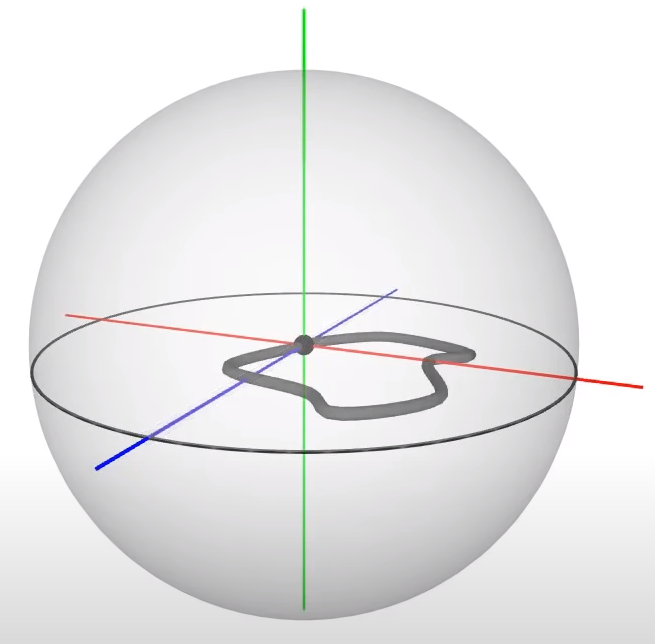
\includegraphics[scale=0.1]{Pictures/randomrotsphere.png} & 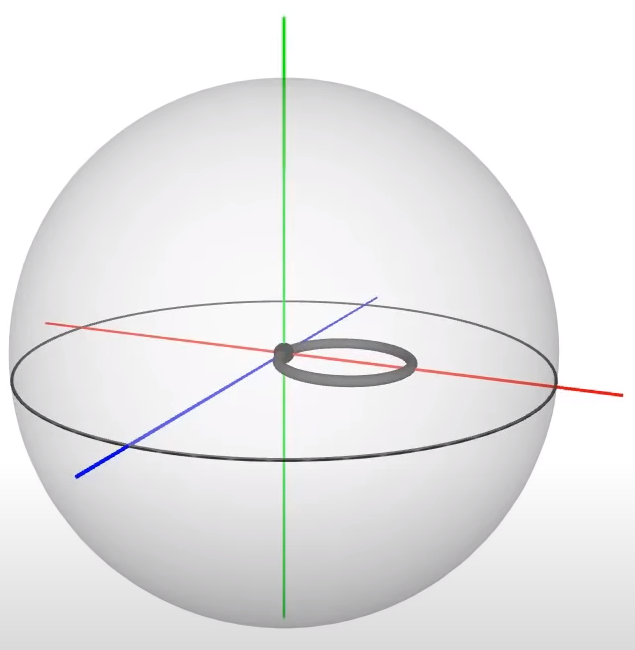
\includegraphics[scale=0.08]{Pictures/contractiblepathsphere.png} & 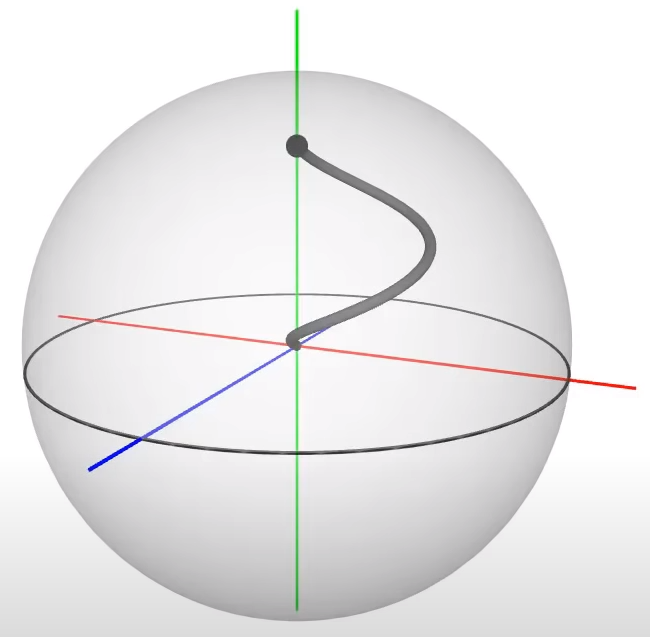
\includegraphics[scale=0.08]{Pictures/noncontractiblepathsphere.png}
    \end{tabular}
    \end{center}
\end{frame}

\begin{frame}{Dictionary}
    We see that:
    \begin{center}
    \begin{tabular}{|ccc|}
        \hline
        \textbf{\underline{Belt}} & & \textbf{\underline{Path}} \\[0.2cm]
        specific configuration & $\longleftrightarrow$ & specific path \\[0.2cm]
        moving the ends & $\longleftrightarrow$ & continuous deformation  \\[0.2cm]
        ends have same orientation & $\longleftrightarrow$ & loop \\[0.2cm]
        \emph{can be flattened} & $\longleftrightarrow$ & \emph{contractible} \\ \hline
    \end{tabular}
    \end{center}
    \textbf{Back to Dirac's belt trick:} the rules were
    \begin{enumerate}
        \item ends of the belt must keep the same orientation \textcolor{blue}{$\to$ we consider loops} \\
        \item moving the ends of the belt \textcolor{blue}{$\to$ continuous deformation} \\
        \item belt in original (flat) position \textcolor{blue}{$\to$ trivial constant path}
    \end{enumerate}
    The question ``can the belt be flattened ?'' then becomes  ``\textbf{which loops are contractible ?}``
\end{frame}

\begin{frame}{Problem solved ?}
    \begin{itemize}
        \item \textbf{\underline{$4\pi$-twist:}}
    We saw in the beginning the the $4\pi$-twist can be flattened, how can we see this in terms of paths ?
    \begin{center}
        \begin{tabular}{m{2cm} m{0.5cm} m{2cm} m{0.5cm} m{2cm}}
            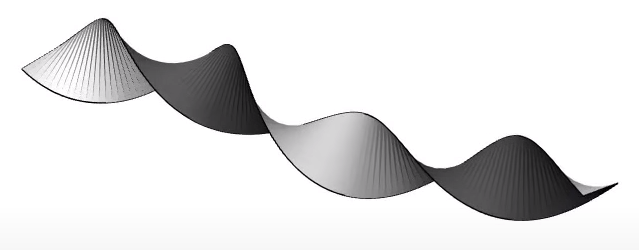
\includegraphics[scale=0.1]{Pictures/4pibelt.png} & $\longleftrightarrow$ & 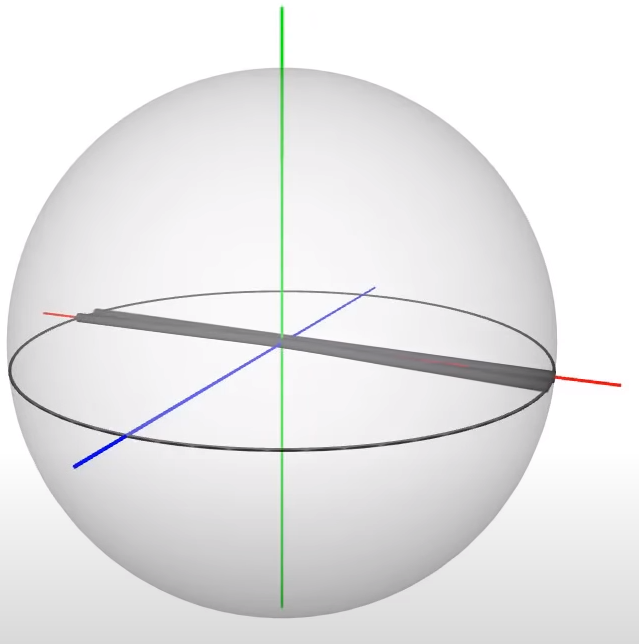
\includegraphics[scale=0.08]{Pictures/4pisphere1.png} & $\longrightarrow$ & 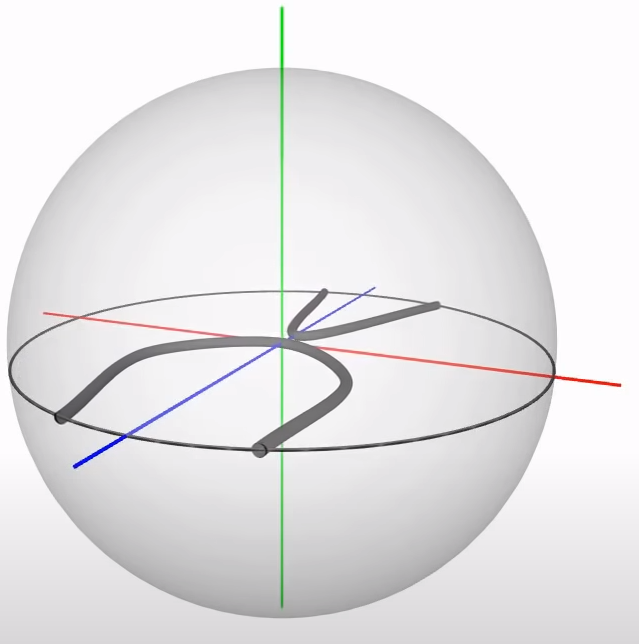
\includegraphics[scale=0.08]{Pictures/4pisphere2.png} \\
            & & & & \hspace{0.7cm} $\downarrow$ \\
            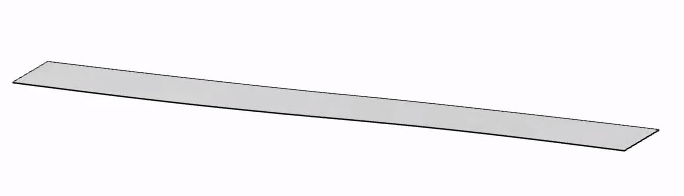
\includegraphics[scale=0.1]{Pictures/flatbelt.png} & $\longleftrightarrow$ & 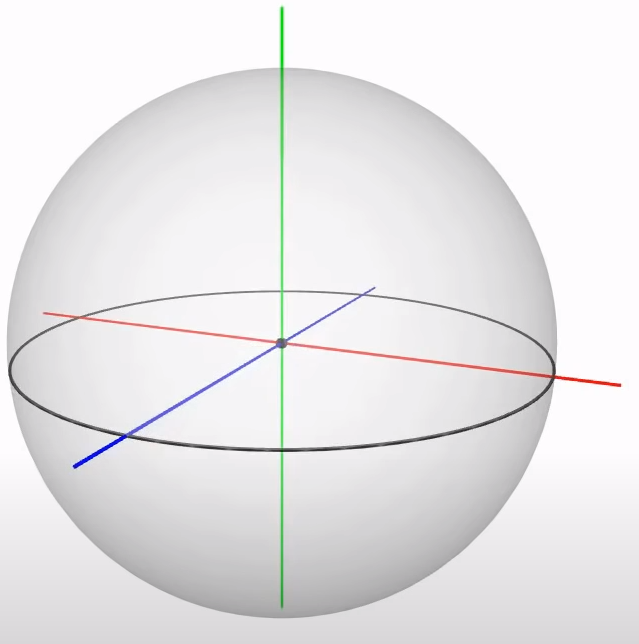
\includegraphics[scale=0.08]{Pictures/4pisphere4.png} & $\longleftarrow$ & 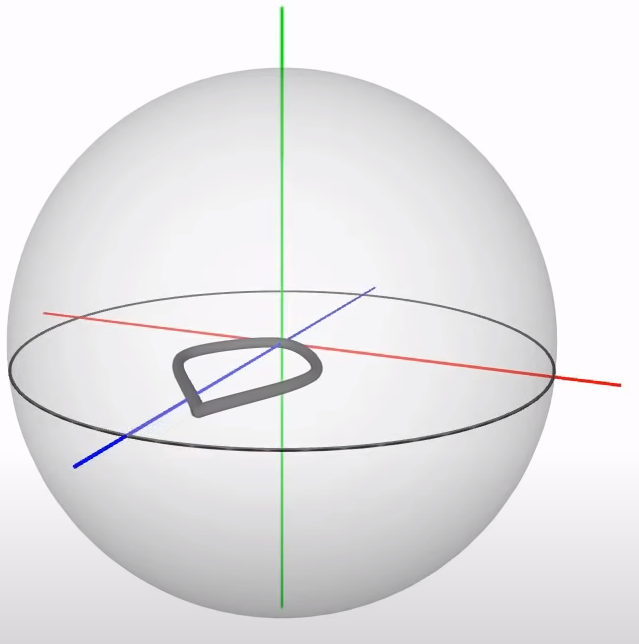
\includegraphics[scale=0.08]{Pictures/4pisphere3.png}
        \end{tabular}
    \end{center}
    $\Rightarrow$ the $4\pi$-twist is \emph{contractible} ! Great.
    \item \textbf{\underline{$2\pi$-twist:}} we ``clearly'' see that is not contractible... no ?! Great..?..  \\[0.2cm]
    \end{itemize}
    \textbf{Wierd aftertaste:} our ``proof'' is good to show contractibility but bad to show non-contractibility and it only works for simple examples.\\
    $\Rightarrow$ We want a consistent and general way of studying paths in topological spaces.
\end{frame}

\section{Homotopy theory}

\begin{frame}{Homotopoy theory primer}
    \textbf{Starting observation:} depending on the topological space, all loops might not be contractible. Moreover, some loops are ``fundamentally different'' from each other, e.g. in $\R^3$, $S^2$, $\mathbb{T}^2$, etc.

    \begin{block}{Paths and homotopies}
        For a topological space $X$:
        \begin{itemize}
            \item \textit{Path} in $X$: continuous map $\gamma:[0,1]\to X$,
            \item \textit{Loop} : closed path, i.e. embedded circle,
            \item $\gamma_1$ and $\gamma_2$ are \textit{homotopically equivalent} if one can be deformed into the other: there exists
            $F:[0,1]\times [0,1]\to X$ such that
            \begin{equation*}
                F(0,t)=\gamma_1(t)\qquad \text{and}\qquad F(1,t)=\gamma_2(t).
            \end{equation*}
            This is an equivalence relation ($\sim$).
        \end{itemize}
    \end{block}
    
    For each $x_0\in X$, we define
    \begin{equation*}
        \boxed{\pi_1(X,x_0) = \{\text{all loops based at }x_0\}/\sim,}
    \end{equation*}
    $\to$ set of ``fundamentally different'' loops passing through $x_0$.
\end{frame}

\begin{frame}{Fundamental group}
    The elements of $\pi_1(X,x_0)$ are $[\gamma]$, called the \textit{homotopy class} of $\gamma$.\\[0.2cm]
    Group structure on $\pi_1(X,x_0)$:
    \begin{itemize}
        \item \textbf{Product} of paths: $\gamma_1\cdot\gamma_2=$ ``$\gamma_1$ then $\gamma_2$''
        \item \textbf{Inverse} path: $\gamma^{-1}=$ ``$\gamma$ traversed in the opposite direction''
        \item \textbf{Neutral} path: $e=$ ``constant path at the identity''
        \item For homotopy classes: $[\gamma_1]\cdot[\gamma_2]=[\gamma_1\cdot\gamma_2]$ and $[\gamma]^{-1}=[\gamma^{-1}]$
    \end{itemize}
    Important fact: if $X$ is path-connected, $\pi_1(X,x_0)$ does not depend on $x_0$, up to isomorphism. \\ $\Rightarrow$ we denote it as $\pi_1(X)$, it is called the \emph{fundamental group} of $X$.\\[0.2cm]
    
    Contractible loops are $\sim$ to a point, i.e. they are the element of $[e]$.\\[0.2cm]

    \begin{block}{Proposition (product of spaces)}
        If $X$ and $Y$ are path-connected, $\pi_1(X\times Y)\cong\pi_1(X)\times\pi_1(Y)$.
    \end{block}
    \begin{block}{Proposition (maps between spaces)}
        If $\vp:X\to Y$ is a continuous map, is induces a homomorphism $\vp_*:\pi_1(X,x_0)\to\pi_1(Y,\vp(x_0))$ though $\vp_*([\gamma])=[\vp\circ\gamma]$.
    \end{block}

\end{frame}

\begin{frame}{Fundamental group}

    Which space have the same fundamental groups ? Evidently, homeomorphic ones, but we can be less restrictive:
    \begin{block}{Proposition}
        If $\vp:X\to Y$ are is a homotopy equivalence, then the induced homomorphism $\vp_*:\pi_1(X,x_0)\to\pi_1(Y,\vp(x_0))$ is an isomorphism for all $x_0\in X$.
    \end{block}

    How to compute $\pi_1(X)$ ? Can be difficult, there a different methods (e.g. Van Kampen theorem, Hopf fibrations, Hurewicz theorems, etc), not discussed here. A lot of homotopy groups are still unknown !\\[0.2cm]

    \begin{columns}[T,onlytextwidth]
        \column{0.55\textwidth}
        
            \textbf{Examples:}\pencil
            {\small
            \begin{itemize}
                \item $\pi_1(\R^3)=0$
                \item $\pi_1(S^2) = 0$
                \item $\pi_1(\mathbb{T}^2)=\pi_1(S^1)\times\pi_1(S^1)=\textcolor{green}{\Z}\times\textcolor{red}{\Z}$
                \item $\pi_1(\R^2\backslash\{p\})=\Z$
            \end{itemize}}
  
        \column{0.45\textwidth}
  
            \begin{figure}
                \centering
                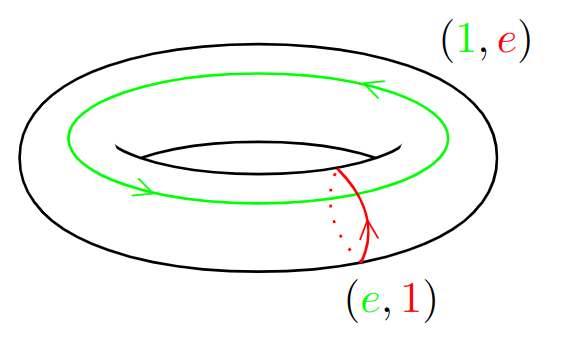
\includegraphics[scale=0.2]{Pictures/torushomotopy3.png}
            \end{figure}
  
    \end{columns}

    Remark: $\pi_1(\R^2\backslash\{p\})=\Z$ but $\pi_1(\R^3\backslash\{p\})=0$, higher homotopy groups for higher-dimensional holes ?
\end{frame}

\begin{frame}{Fundamental group of the circle}

    Using the covering space technology, we can show that
    \begin{equation*}
        \boxed{\pi_1(S^1)=\Z,}
    \end{equation*}
    which intuitively make sense. This results alone implies many famous theorems of topology:
    \begin{block}{Theorem (fundamental theorem of algebra)}
        Every non-constant polynomial with coefficients in $\C$ has a root in $\C$.
    \end{block}
    \begin{block}{Theorem (Brouwer fixed point)}
        Every continuous map $h:D^2\to D^2$ has a fixed point.
    \end{block}
    And, using the same techniques:
    \begin{block}{Theorem (Borusk-Ulam)}
        For every continuous map $f=S^2\to \R^2$ there exist a pair of antipodal points $x$ and $-x$ in $S^2$ such that $f(x)=f(-x)$.
    \end{block}

    One can generalize and show that $\pi_n(S^n)=\Z$. These theorems are then generalized accordingly.
    
\end{frame}

\begin{frame}{Homotopy groups of spheres}

    Good example of the complexity of homotpy groups:\\[0.2cm]
    \quad $\triangleright$ embedding a sphere in a higher-dimensional one is always trivial \\[0.2cm]
    \quad $\triangleright$ embedding a sphere in itself always works in the same way,\\ \hspace{0.5cm} regardless of the dimension \\[0.2cm]
    \quad $\triangleright$ embedding a sphere in lower-dimensional one is much more \\ \hspace{0.5cm} complicated: periodic for a bit, then completely chaotic

    \begin{figure}
        \centering
        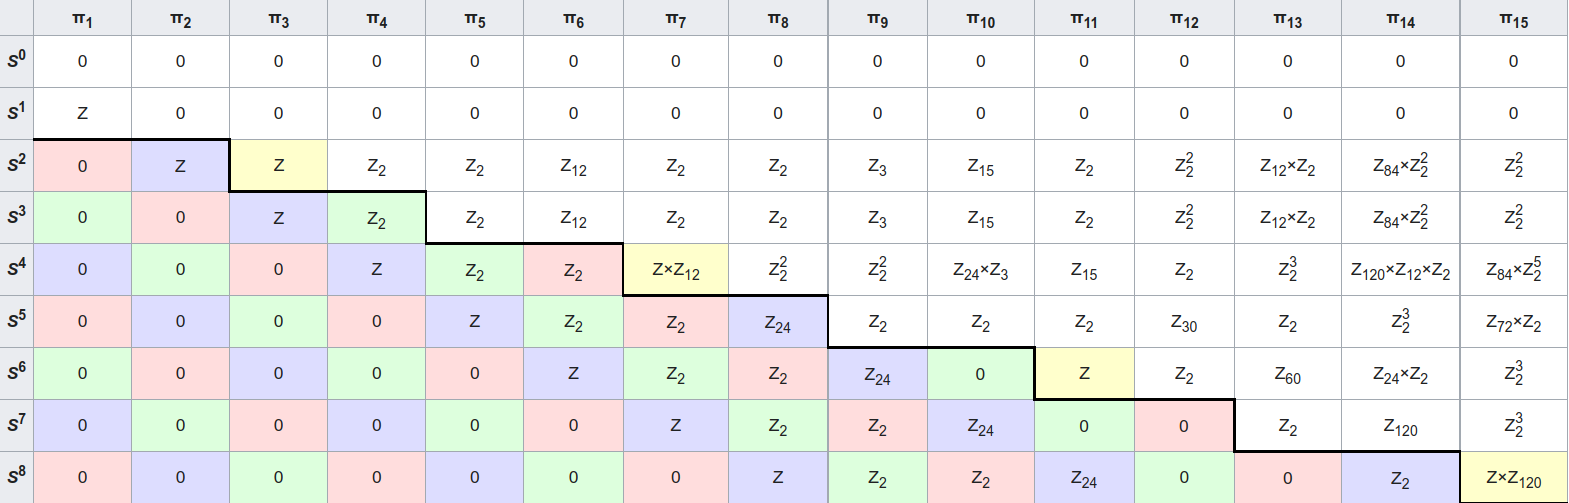
\includegraphics[scale=0.2]{Pictures/homotpoygroupsphere.png}
    \end{figure}


\end{frame}

\begin{frame}{Back to $\SO(3)$}
    \textbf{Question we had:} are all loops in $\SO(3)$ contractible ?\\
    In homotopy language: is $\pi_1(\SO(3))$ trivial ?\\[0.2cm]
    \textbf{Answer:} \emph{NO}, one can show that
    \begin{equation*}
        \boxed{\pi_1(\SO(3))=\Z_2}
    \end{equation*}
    $\Rightarrow$ There only two ``fundamentally different'' loops in $\SO(3)$ !\\
    $\Rightarrow$ there is only one kind of non-contractible loop !

    \begin{center}
        \begin{tabular}{|l|}
            \hline
            The belt trick is a way of physically demonstrating that the \\ fundamental group of $\SO(3)$ is $\Z_2$.\\ \hline
        \end{tabular}
    \end{center}
    Indeed, there only two different initial configurations (i.e. two possible loops in $\SO(3)$):
    \begin{itemize}
        \item $4\pi k$-twists which are all equivalent
        \item $4\pi k+2\pi$-twists which are all equivalent
    \end{itemize}
    with $k\in\Z$.\\[0.2cm]

    We have a better understanding Dirac's belt trick. \textbf{But still no proof !} Homotopy theory allowed us to understand the ways of embedding loops in some spaces, we now need a tool to lift this ambiguity: \emph{covering space} !

\end{frame}

\section{Covering spaces}

\begin{frame}{Covering spaces}
    
    \begin{columns}[T,onlytextwidth]
        \column{0.75\textwidth}
        
            \begin{block}{Covering space}
                For a topological space $X$, a \textit{covering space} is a topological space $\tilde{X}$ with a \textit{projection map} $p=\tilde{X}\to X$ such that there exists an open cover $\{\U_\alpha\}$ for which $p^{-1}(U_\alpha)$ is a disjoint union of open sets in $\tilde{X}$, each of which is mapped by $p$ homeomorphically on $U_\alpha$. \\
                If $X$ is connected, $|p^{-1}(x)|$ is constant and called the number of \textit{sheets}.
            \end{block}
  
        \column{0.25\textwidth}
  
            \begin{figure}
                \centering
                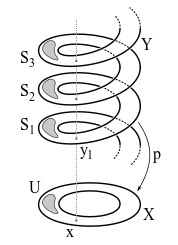
\includegraphics[scale=0.4]{Pictures/Covering_map.png}
            \end{figure}
  
    \end{columns}

    \textbf{Example:} covering the circle. Many possibilities:\pencil
        \begin{itemize}
            \item $\R$ covers $S^1$ with $p(t)=(\cos(2\pi t),\sin(2\pi t))$,
            \item $\R$ covers $S^1$ with $p(t)=(\cos(5 t),\sin(5 t))$,
            \item $S^1$ covers $S^1$ in several ways, with $p(z)=z^n$, $n\in\N$,
            \item $S^1\sqcup S^1$ covers $S^1$ with $p(k,t)=t$, $k=0,1$.
        \end{itemize}
    

\end{frame}

\begin{frame}{Important notions}

    We observe that
    \begin{enumerate}
        \item \textbf{Some covering spaces are ``equivalent'':}
            \begin{minipage}{10cm}
                \begin{block}{Isomorphisms}
                    Two covering space $\tilde{X}$ and $\tilde{X}'$ of $X$ are \textit{isomorphic} if there exists a homeomorphism $h:\tilde{X}\to \tilde{X}'$ such that $p_2\circ h=p_1$.
                \end{block}
            \end{minipage}
        \item \textbf{The lifting of point can, by definition, be ambiguous.}
            \begin{minipage}{10cm}
                \begin{block}{Deck transformations}
                    A \textit{Deck transformation} is a homeomorphism $d:\tilde{X}\to \tilde{X}$ such that $p\circ d=p$. With composition, they form a group $G(\tilde{X})$.
                \end{block}
            \end{minipage}
            \textcolor{blue}{For $S^1$, $G(\R)=\Z$ and $G(S^1)=\Z_n$.}
        \item \textbf{Some covering spaces are ``included`` in others:} we restrict ourselves to connected covering spaces.
            
        \item \textbf{There can exists many covering spaces for the same base space.} If $\tilde{X}$ is simply connected and $X$ is (locally) path-connected, then it is a covering space of any other covering space. It is maximal, unique and called \textit{universal covering space} (UCS). \textcolor{blue}{$\R$ is the UCS of $S^1$.}
    \end{enumerate}

\end{frame}

\begin{frame}{Covering spaces and paths}
    \begin{columns}[T,onlytextwidth]
        \column{0.7\textwidth}
        
            \begin{block}{Lifting property of paths}
                For each path $\gamma:I\to X$ starting at $x_0$, if we fix $\tilde{x}_0\in p^{-1}(x_0)$, there is unique lifted path $\tilde{\gamma}:I\to \tilde{X}$ starting at $\tilde{x}_0$.
            \end{block}
            
            We see that:\\
            \quad $\triangleright$ loop are not necessarily lifted to loops\\
            \quad $\triangleright$ the lift of a constant path is still constant\\
            Most importantly : the lifts of homotopy-equivalent paths are homotopically equivalent.


  
        \column{0.3\textwidth}
  
        \begin{figure}
            \centering
            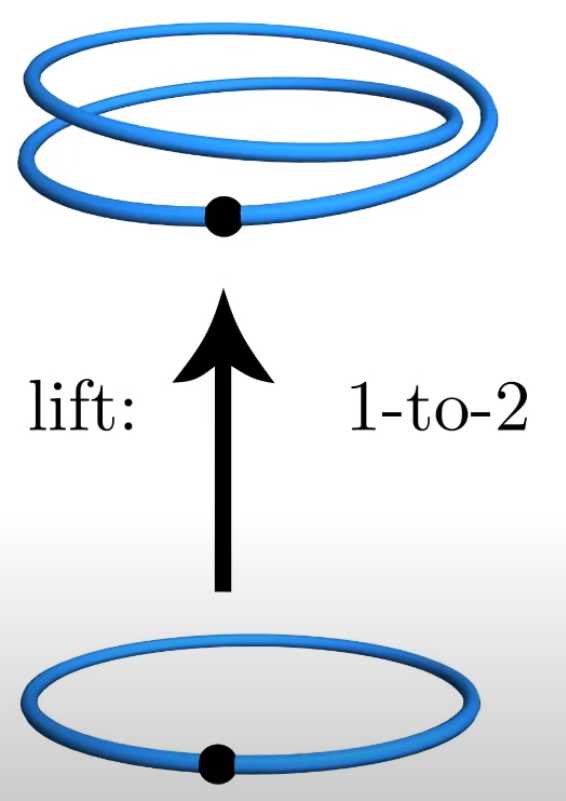
\includegraphics[scale=0.1]{Pictures/lifting_point.png}
        \end{figure}
        \begin{figure}
            \centering
            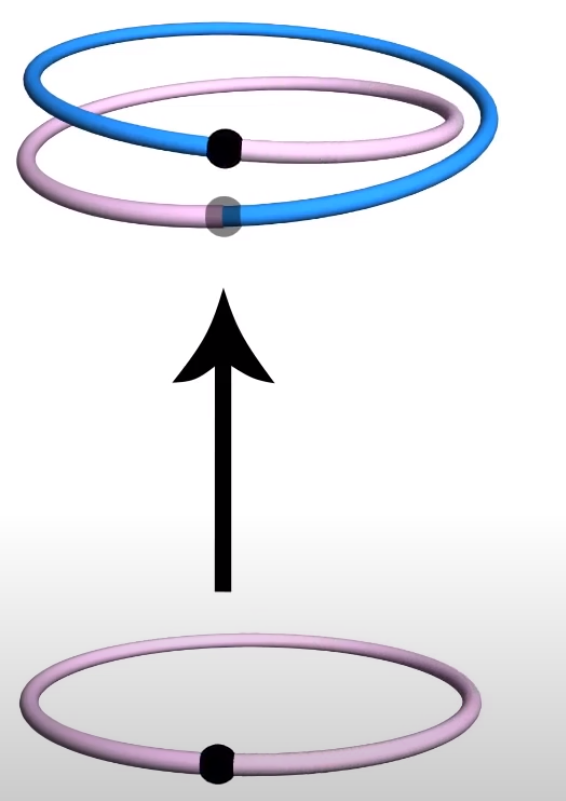
\includegraphics[scale=0.1]{Pictures/lifting_path.png}
        \end{figure}
  
    \end{columns}

    The covering is exactly what solves the homotopy ambiguity, i.e. the space that contains the same infirmation plu the the topological information of non-equivalent paths!

    \emph{Conclusion:} the fundamental group and the covering space are two pictures of the same thing: algebraic features of $\pi_1(X)$ can be seen as geometric features of $\tilde{X}$.
\end{frame}

\begin{frame}{Covering space of $\SO(3)$ ?}
    \begin{block}{Special unitary group}
        $\SU(2)$ is the set of $2\times 2$ complex matrices such that $U^\dagger U=\mathbbm{1}$ and $\det U=1$.
    \end{block}
    \begin{figure}
        \centering
        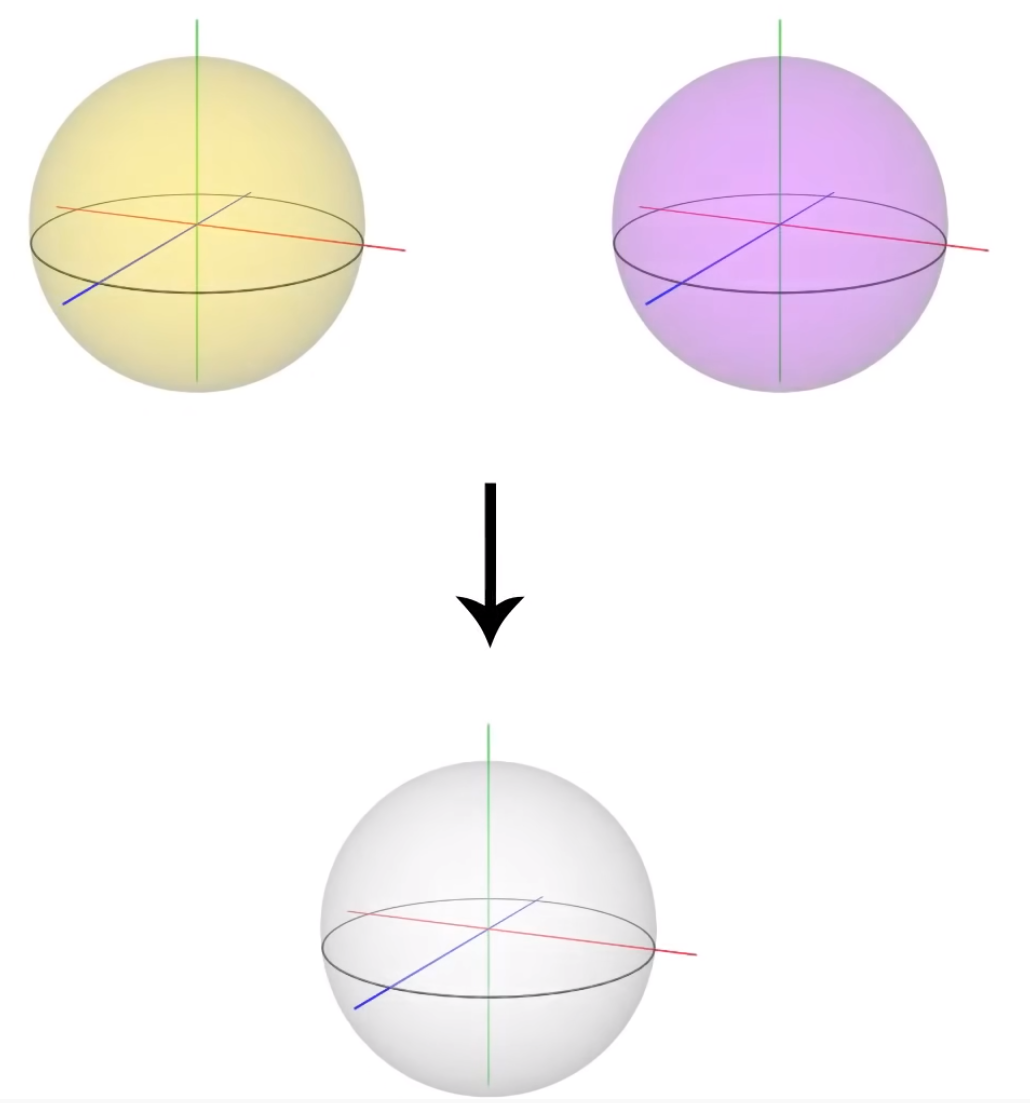
\includegraphics[scale=0.1]{Pictures/lifting_su2.png}
    \end{figure}
    The projection is
    \begin{equation*}
        p\left(\begin{bmatrix}
            x & y \\
            -\bar{y} & \bar{x}
        \end{bmatrix}\right)=
        \begin{bmatrix}
            \Re(x^2-y^2) & \Im(x^2+y^2) & -2\Re(xy) \\
            -\Im(x^2-y^2) & \Re(x^2+y^2) & 2\Im(xy) \\
            2\Re(x\bar{y}) & 2\Im(x\bar{y}) & \abs{x}^2-\abs{y}^2
        \end{bmatrix}
    \end{equation*}
    with $\abs{x}^2+\abs{y}^2=1$.
\end{frame}

\begin{frame}{$\SU(2)$ and $\SO(3)$}
    What is the most general for of $U\in\SU(2)$ ? Imposing $U^\dagger=U^{-1}$ and $\det U=1$, we find
    \begin{equation}
        U=
        \begin{bmatrix}
            X+iY & Z+iW \\
            -Z+iY & X-iY
        \end{bmatrix}
    \end{equation}
    with $X^2+Y^2+Z^2+W^2=1$ $\Rightarrow \SU(2)\cong S^3$\\
    so $\SU(2)$ can be viewed as a group and a manifold, it is a Lie group\\[0.2cm]
    $\SU(2)$ and $\SO(3)$:
    \begin{enumerate}
        \item both Lie groups of dimension three
        \item both are connected
        \item $-\mathbbm{1}\in\SU(2)$ but $-\mathbbm{1}\notin\SO(3)$
    \end{enumerate}
    How could we represent $\SU(2)\cong S^3$ in $3d$ ?\\[0.2cm]
    Observation: $S^2$ is equivalent to two disks glued along their boundary\\[0.2cm]
    Similarly: $S^3$ is equivalent to balls glued along their boundary\\[0.2cm]
    \textbf{BUT}, are those spheres related to $\SO(3)$ ?\\
    In other words: how are the two notions of rotations related ? They are the sheets! \\[0.2cm]
\end{frame}


\begin{frame}{Last comments on $\SU(2)$ and $\SO(3)$}
    \textbf{\underline{Group relation:}}\\[0.2cm]
    There is recurring theme: two things $\SU(2)$ correspond to one in $\SO(3)$. This comes from the fact that $\SU(2)$ is a \emph{double}-cover of $\SO(3)$, which can can see in practice with
    \begin{equation*}
        p(U)=p(-U).
    \end{equation*}
    Intuitively, we should be able to recover $\SO(3)$ from $\SU(2)$ if $U\sim-U$.\\[0.2cm]
    And, indeed,
    \begin{equation*}
        \SO(3)\cong\SU(2)/\Z_2,
    \end{equation*}
    where the quotient means exactly that we identity $U$ with $-U$.\\[0.2cm]

    \textbf{\underline{Other formulation:}}\\[0.2cm]

    $S^3$ is a universal double-sheeted cover of $\R\P^3$, $\pi_1(S^3)=\{e\}$, and $\pi_1(\R\P^3)=\Z_2$. This formulation makes a lot of sense since $\R\P^3=S^3/\{(x,y,z)\sim(-x,-y,-z)\}$, or $\R\P^3=S^2/\Z_2$, so exactly get the previous group relation.

\end{frame}

\begin{frame}{Summary on $\SU(2)$ and $\SO(3)$}
    \begin{enumerate}
        \item $\SU(2)$ is the universal covering space of $\SO(3)$, it has two sheets
        \item we can construct an explicit projection map
        \item we, finally, completely understand Dirac's belt trick
        \item ...
    \end{enumerate}
    
\end{frame}

\begin{frame}{Bringing it all together}
    What is the lift of the $2\pi$-twist ? The path going from $I$ to $-I$ \pencil\\[0.2cm]
    \textbf{\underline{Proof that $2\pi$-twist is non-contractible in $\SO(3)$:}}
    \begin{flushright}
    \begin{minipage}{10.5cm}
        Let us suppose that the $2\pi$-twist is contractible. At each step of its contraction, we can lift the path to $\SU(2)$. This provides us with a contraction of the lifted $2\pi$-twist. However, the lifted $2\pi$-twist does not have the same start and endpoint, therefore it is not contractible, and so is the non-lifted path.
    \end{minipage}
    \end{flushright}
    On the other hand, the $4\pi$-twist lifts to a path going from $I$ to $-I$ then to $I$ again (\pencil). So its a loop and the argument does not hold anymore. Makes sense, since we already ``showed'' its contractibility.\\[0.2cm]

    Are there other manifestation of homotopy in our practical world ?\\[0.2cm]

    Yes: the \emph{spin} ! (you don't need a belt, but you need an electron)\\[0.2cm]
    Initially, this trick was a demonstration invented by P. Dirac (1902-1984) to explain the notion of spin to his students.
\end{frame}


\section{Quantum spin}

\begin{frame}{Rotating a spin vector}
    \textbf{\underline{For vectors:}} recall that the scalar product on $\R^3$ is $\langle v_1,v_2\rangle_{\R^3}=(v_1)^Tv_2$ and
    \begin{equation*}
        \langle Rv_1,Rv_2\rangle_{\R^3} = \langle v_1,v_2\rangle_{\R^3}\qquad \Leftrightarrow\qquad R^T R = \mathbbm{1}
    \end{equation*}
    so $\SO(3)$ is the isometry group of $\R^3$ (+ orientation preserving).\\[0.2cm]
    \textbf{\underline{For spin vectors:}} the scalar product on $\C^2$ is $\langle v_1,v_2\rangle_{\C^2}=(v_1)^\dagger v_2$ and
    \begin{equation*}
        \langle Uv_1,Uv_2\rangle_{\C^2} = \langle v_1,v_2\rangle_{\C^2}\qquad \Leftrightarrow\qquad U^\dagger U = \mathbbm{1}
    \end{equation*}
    so $\SU(2)$ is the isometry group of $\C^2$ (+ orientation preserving).\\[0.2cm]
    Like $\SO(3)$ it is a Lie group so it can be viewed...
\end{frame}

\begin{frame}{What is the spin ?}

    Skipping most of the physics background:
    \begin{block}{Spin in quantum mechanics}
        \begin{enumerate}
            \item the \textit{spin}  is an inherent property of any ``particle'':
            \begin{itemize}
                \item number $s\in\frac{1}{2}\N$\textcolor{blue}{, in our case $s=1/2$}
                \item does not change, like the mass, charge, etc
                \item classifies particles
            \end{itemize}
            \item a particle of spin $s$ is, at a given moment, in a certain state described by the \textit{spin vector}:
            \begin{itemize}
                \item unit vector of $v\in\C^{2s+1}$\textcolor{blue}{, in our case $\begin{bmatrix}\alpha\\ \beta\end{bmatrix}\in\C^2$}
                \item can evolve over time
            \end{itemize}
            \item what we can measure yet another quantity, called \textit{observed spin}:
            \begin{itemize}
              \item discrete value $s_{\text{obs.}}\in\{s,s-1,\dots,0,\dots,-s+1,-s\}$\\
              \textcolor{blue}{In our case, $s_{\text{obs.}}\in\{1/2,-1/2\}$ that we denote $\uparrow$ and $\downarrow$}
              \item given a direction, e.g. $i=x,y,z$
              \item outcome is random, we can only compute de probabilities of the different outcomes
            \end{itemize}
        \end{enumerate}
    \end{block}

\end{frame}

\begin{frame}{What is the spin ?}
    \textbf{How do measures happen ?}\\[0.2cm]
    Let us introduce
    {\small
    \begin{align*}
        v_{x,\uparrow}=
        \begin{bmatrix}
            1/\sqrt{2} \\ 1/\sqrt{2}
        \end{bmatrix},
        v_{x,\downarrow }=
        \begin{bmatrix}
            1/\sqrt{2} \\ -1/\sqrt{2}
        \end{bmatrix},
        v_{y,\uparrow}=
        \begin{bmatrix}
            1/\sqrt{2} \\ i/\sqrt{2}
        \end{bmatrix},
        v_{y,\downarrow}=
        \begin{bmatrix}
            1/\sqrt{2} \\ -i/\sqrt{2}
        \end{bmatrix},
        v_{z,\uparrow}=
        \begin{bmatrix}
            1 \\ 0
        \end{bmatrix},
        v_{z,\downarrow}=
        \begin{bmatrix}
            0 \\ 1
        \end{bmatrix}.
    \end{align*}}
    The probability of measuring $s_{\text{obs.}}$ in the direction $i$ is given by the projection
    \begin{equation}
        P(i,s_{\text{obs.}}) = \abs{\langle v_{i,k},v \rangle_{\C^2}}^2
    \end{equation}
    where $v$ is the spin vector of the particle.\\[0.2cm]
    \textbf{Example}: in the direction $z$,
    \begin{equation}
      P(z,\uparrow)= \abs{\alpha}^2,\qquad P(z,\downarrow)= \abs{\beta}^2.
    \end{equation}
    Consequently:
    \begin{itemize}
        \item we must have $\langle v,v\rangle_{\C^2}=\abs{\alpha}^2+\abs{\beta}^2=1$
        \item to ``measure'' the spin state, we must repeat the experience many times
        \item there are states that are always spin $\uparrow$ or always spin $\downarrow$
    \end{itemize}
\end{frame}

\begin{frame}{Generalization to other spins}
    % we discussed something for in three dimensions (with SO(3) and SU(2)), how can we generalize this ?
    % motivation: any rotation in R^3 can be achived in two topologically inequivalent ways, why should objects be blind to that ? The most general object is spinors
    % how to distinguish the topologically inequivalent rotations ? Universal cover of the group, double cover, spin groups
    % properties of the spin groups; in any dimension, actully always TWO topologically inequivalent ways of achieving a rotation, i.e. it is always a DOUBLE cover, it is unique, maximal, etc
    % def of spinor
    % other definition of spinor: Clifford algebras, def the algebra
    % link with the other definition: Both the spin group and its Lie algebra are embedded inside the Clifford algebra in a natural way, and in applications the Clifford algebra is often the easiest to work with.
    % representation theory of the CLifford algebra, i.e. spinors in all dimensions
    % come back the three dimensions, our example of SU(2) etc, with representations theory of SO(3) and SU(3), integer spin and half-interger spins

    % there are essentially two frameworks for viewing the notion of a spinor.

    % ccl the integer spin particles are vector repr (called bosons), they don't care about the homotopy class, the half integer spins are proper spinors, they caeer about the homotopy class, they are sensible to an additional Z_2 (called fermions).
\end{frame}

\begin{frame}{The bizarre nature of fermions}
    The group which acts on spin vectors is $\SU(2)$.\\[0.2cm]
    \textbf{Question:} how do rotations act on spin vectors ? The rotation group of euclidean space is still $\SO(3)$, so we need a way of doing an $\SO(3)$ rotation through $\SU(2)$ transformations.\\[0.2cm]
    This is exactly what the covering technology provides us: a unique way to lift a rotation from $\SO(3)$ to $\SU(2)$.\\[0.2cm]
    The $2\pi$-twist is not closed $\Rightarrow$ walking around such a particle would not give back the particle in the same states, it would inverts the spin state.\\[0.2cm]
    \textbf{But}, very odd property ... could such exotic particles exist ? Or is it an error of interpretation ?\\[0.2cm]
    \emph{Yes}, they do exist! Out of the $18$ elementary particles, $12$ of them have spin $1/2$ ! And this have been experimentally 
\end{frame}

\begin{frame}{Elementary particles}
    \begin{figure}
        \centering
        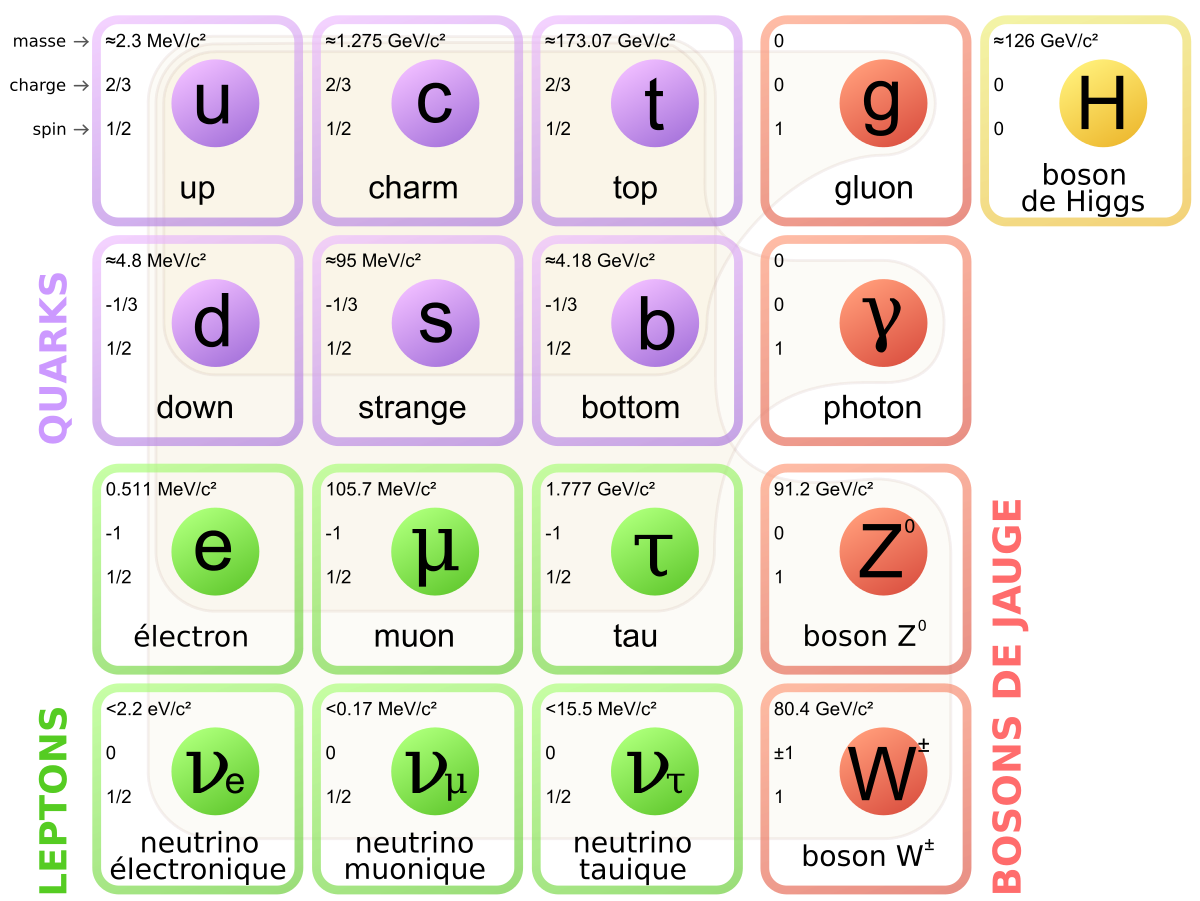
\includegraphics[scale=0.22]{Pictures/SM.png}
        \caption{Standard Model of particle physics.}
    \end{figure}
\end{frame}

\begin{frame}{Remarks}

    \begin{columns}[T,onlytextwidth]
        \column{0.5\textwidth}
          
        \textbf{\underline{Technical details:}}
        \begin{itemize}
            \item instead of walking around the particle, we rotate it using a magnetic field (Lamor procession)
            \item we cannot detect the effect if there only one particle
            \item we do not actually use electrons but neutrons (see neutron interferometry).
        \end{itemize}
        \textbf{\underline{Spin in nature:}}
    
        \column{0.5\textwidth}
    
            \begin{figure}
                \centering
                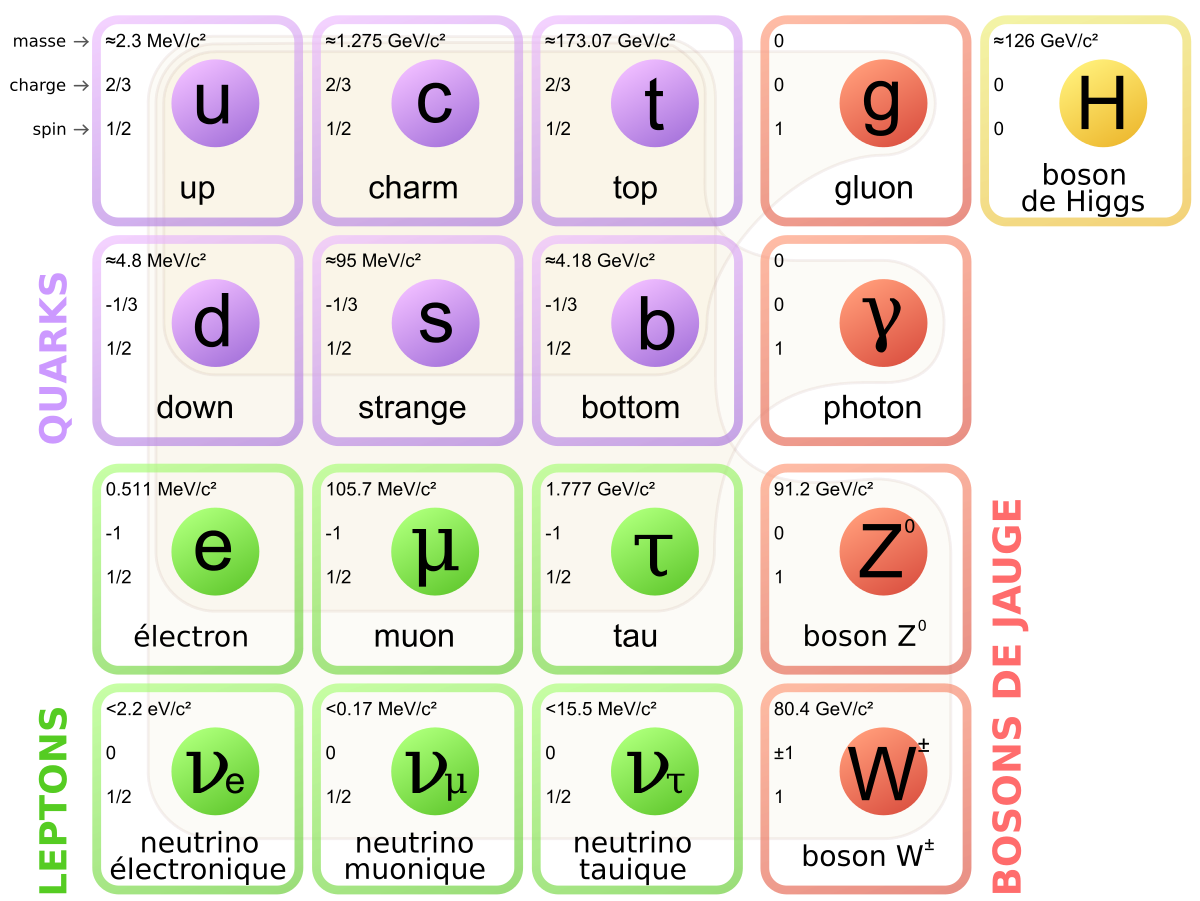
\includegraphics[scale=0.12]{Pictures/SM.png}
                \caption{Standard Model of particle physics.}
            \end{figure}
    
    \end{columns}

    
    \begin{itemize}
        \item in nature, only spins $0$ (Higgs boson), $1/2$ (electrons, quarks, etc), $1$ (photons, gluons, etc) and $2$ (graviton)
        \item spins higher than $2$ are very problematic, and not well-understood yet. Current topic of research (UMons !)
        \item spin-$1/3$ particles ? No, impossible, because $\pi_1(SO(3))=\Z_{\textcolor{red}{2}}$. Example of mathematical constraint on physical models.
    \end{itemize}
     modern fundamental physics is relativistic so we use a pseudo-scalar product. The isometry group becomes $\SO(1,3)$. The spinor theory we depicted can be generalized to $\SO(p,q)$.

\end{frame}

\begin{frame}{Remarks}
    \textbf{\underline{Behind quantum mechanics:}} \\[0.2cm]

    The spinors we encountered previously are spinors in Quantum Mechanics, which is non-relativistic. Modern Physics is relativistic therefore we mainly care about the indefinite rotation groups rather than the usual rotation groups, because of special relativity. The whole theory can be generalized accordingly.

    \begin{figure}
        \centering
        \begin{tabular}{c|cc}
            & \textbf{Non-relativistic} & \textbf{Relativistic} \\ \hline
            rotation group & $\SO(3)$ & $\SO(1,3)$ \\
            UCS & $\Spin(3)=\SU(2)$ & $\Spin(1,3)=\SL(2,\C)$
        \end{tabular}
    \end{figure}

\end{frame}

\begin{frame}{Summary on spinors}
    \begin{enumerate}
        \item There are two topologically distinguishable classes (homotopy classes) of paths through rotations that result in the same overall rotation, as illustrated by the Dirac's belt trick. (True in any dimension.) 
        \item Nothing forces us to consider only objects that do not make this difference (vectors). We should consider the most general case, this is what spinors are.
        \item Spinors change in different ways depending not just on the overall final rotation, but the details of how that rotation was achieved (by a continuous path in the rotation group).
        \item The spin group is the group of all rotations keeping track of the class. It doubly covers the rotation group, since each rotation can be obtained in two in-equivalent ways as the endpoint of a path.
        \item The space of spinors by definition is equipped with a (complex) linear representation of the spin group.
        \item A spinor is characterized by its \emph{spin}. Depending on the dimension of the space, the dimensions of the spin representations vary but all spins are always possible.
    \end{enumerate}
\end{frame}

\begin{frame}{Spinors in relativistic Physics}

    

    
\end{frame}

\section{More belts}

{
\setbeamercolor{background canvas}{bg=black!100}
\begin{frame}{Anti-twister mechanisms}
    \begin{center}
        \movie[width=10cm,height=5.5cm,showcontrols,loop]{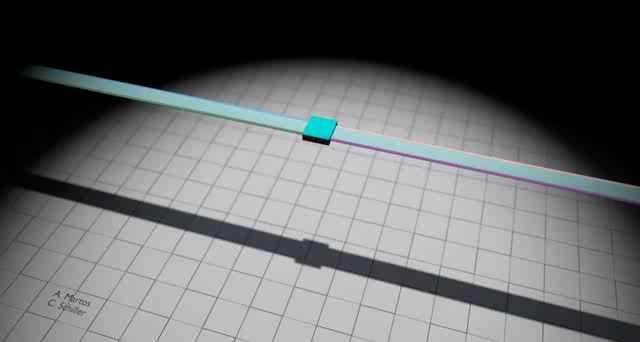
\includegraphics[scale=0.25]{Pictures/poster2belts.jpg}}{Videos/2belts.wmv}
    \end{center}
    {\small\textcolor{white}{Expanding the Dirac's belt trick setup, one can attach two belts to an object and rotate it by 720° without it getting tangled. Combining the two movements,the object can spin continuously without becoming tangled.}}
\end{frame}}

{
\setbeamercolor{background canvas}{bg=black!100}
\begin{frame}{Anti-twister mechanisms}
    \begin{center}
        \movie[width=10cm,height=5.5cm,showcontrols,loop]{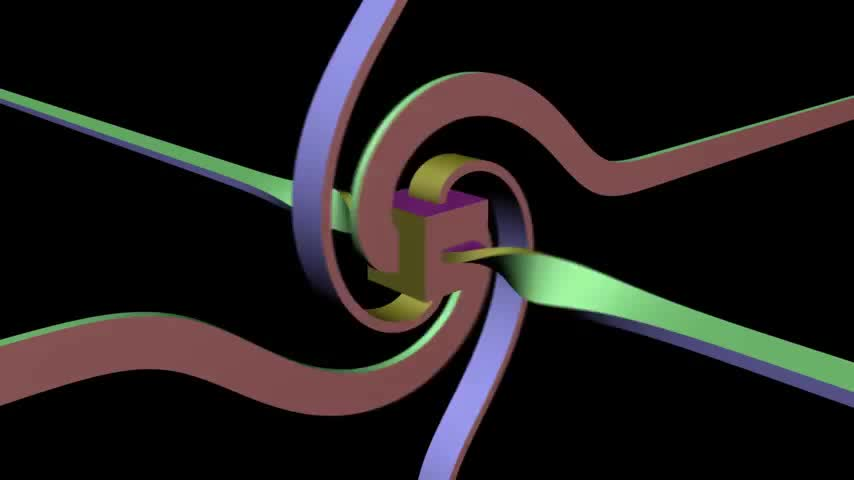
\includegraphics[scale=0.25]{Pictures/poster1.jpg}}{Videos/video1.wmv}
    \end{center}
    {\small\textcolor{white}{Increasing the number of belts does not change this behavior. Notice that after the cube completed a 360° rotation, the spiral is reversed from its initial configuration. It only returns to its original configuration after spinning a full 720°.}}
\end{frame}}

{
\setbeamercolor{background canvas}{bg=black!100}
\begin{frame}{Anti-twister mechanisms}
    \begin{center}
        \movie[width=10cm,height=5.5cm,showcontrols,loop]{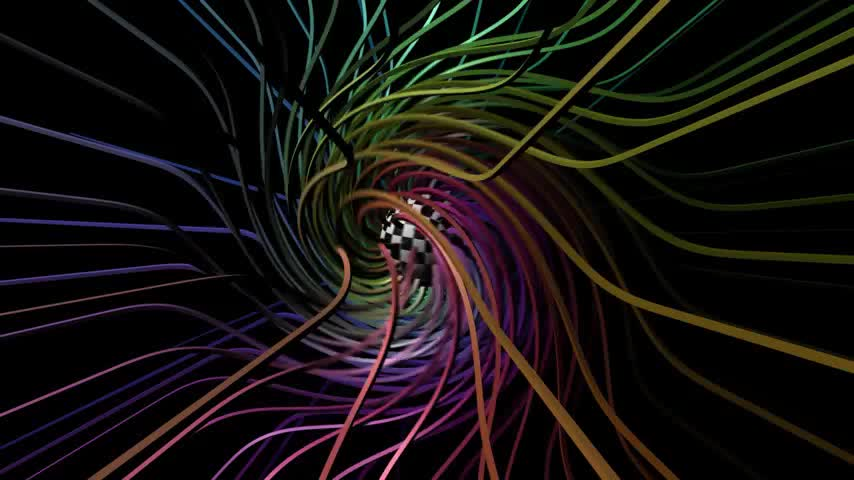
\includegraphics[scale=0.25]{Pictures/poster2.jpg}}{Videos/video2.wmv}
    \end{center}
    {\small\textcolor{white}{A more extreme example demonstrating that this works with any number of strings. In the limit, a piece of solid continuous space can rotate in place like this without tearing or intersecting itself.}}
\end{frame}
}
% https://bloerg.net/posts/beamer-movies-and-linux/



\section{Fun facts}

\begin{frame}{Fun facts}
    \begin{itemize}
        \item anti-twister mechanism is used in engineering to supply electric power to rotating devices
        \item cup on the hand trick (balinese candle dance or Philippine wine dance)
        \item tangloids is mathematical gamed base on the same principles
        \item link with quaternions
    \end{itemize}

    \begin{figure}
        \centering
        \begin{subfigure}[b]{0.5\textwidth}
            \centering
            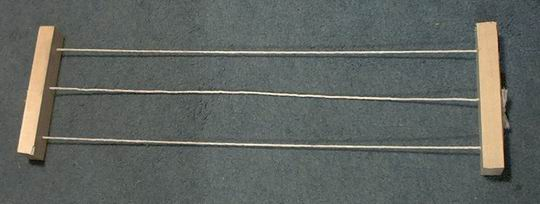
\includegraphics[scale=0.2]{Pictures/Tangloids.jpeg}
            \caption{Tangloids.}
        \end{subfigure}\begin{subfigure}[b]{0.5\textwidth}
            \centering
            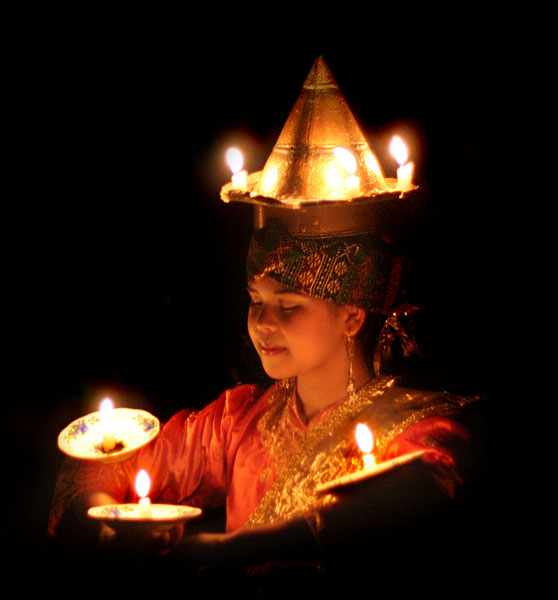
\includegraphics[scale=0.2]{Pictures/balinesedance.jpg}
            \caption{Balinese candle dance.}
        \end{subfigure}
   \end{figure}

   

\end{frame}

% tangloids
% videos on 
% anti-twister mechanism: The anti-twister or antitwister mechanism is a method of connecting a flexible link between two objects, one of which is rotating with respect to the other, in a way that prevents the link from becoming twisted. The link could be an electrical cable or a flexible conduit. This mechanism is intended as an alternative to the usual method of supplying electric power to a rotating device. What makes the device possible is the peculiar connectivity of the space of 3D rotations, as discovered[3] by P. A. M. Dirac and illustrated in his Plate trick (also known as the string trick or belt trick).[4] Its covering Spin(3) group can be represented by unit quaternions, also known as versors.

\section{Conclusion}

\begin{frame}
    \begin{enumerate}
        \item Dirac's belt trick can be understood by studying the fundamental group of $\SO(3)$.
        \item The universal cover of $\SO(3)$ is $\SU(2)$, in which the homotopy ambiguity is solved. Spin vectors transform under $\SU(2)$ and covering space technology then allows us to better understand the nature of the spin in quantum mechanics.
        \item Spinors can be defined in any dimension and for any spin. Leading to a generalization of usual vectors that take into account the topological difference between some rotations that, a priori, could look equivalent.
        \item Spinors are fundamental in Physics and in particular all modern theories of fundamental interactions. Spinors model most of elementary particles. In particular, exactly like Dirac's belt, electrons rotate through the lift in $\SU(2)$ thus taking into account the homotopy class of the rotation, how cool !
    \end{enumerate}
    \vspace{0.5cm}
    \begin{center}
        {\huge\textit{Thank you}}
    \end{center}
\end{frame}


\begin{frame}{Blocks}
    Three different block environments are pre-defined and may be styled with an
    optional background color.
  
    \begin{columns}[T,onlytextwidth]
        \column{0.5\textwidth}
          
            Some text.\\[2cm]
            aaaaa
    
        \column{0.5\textwidth}
    
            \begin{block}{Default}
              Block content.
            \end{block}
      
            \begin{alertblock}{Alert}
              Block content.
            \end{alertblock}
      
            \begin{exampleblock}{Example}
              Block content.
            \end{exampleblock}
    
    \end{columns}

\end{frame}

\appendix

{
\setbeamercolor{background canvas}{bg=green!10}

\begin{frame}{Introduction to the spin}
    
    \begin{block}{Spin in quantum mechanics}
        The \emph{spin} of an ``particle'' is a number $s\in\frac{1}{2}\N$.\\
        The \emph{spin state} of a particle of spin $s$ is a unit vector in $\C^{2s+1}$.
    \end{block}
    The spin is a \emph{property}, it cannot change (e.g. mass, charge)\\
    The spin state is a \emph{characteristic}, it evolves

    How to interpret it ? 
    \begin{enumerate}
        \item \textbf{directions:} we choose the direction in which we want to measure it
        \item \textbf{probabilistic theory:} the outcome of the measure, we can only compute the probabilities of the different outcomes
        \item \textbf{discrete quantity:} in the chosen direction, the spin will either appear to up or down ($\uparrow$ or $\downarrow$)
    \end{enumerate}
    The probability of measuring the spin $k=\uparrow,\downarrow$ in the direction $i=x,y,z$ is given by
    \begin{equation}
        P(i,k) = \abs{\langle v_{i,k},v \rangle}^2
    \end{equation}
    where $v$ is the spin state of the particle, for some given vectors $v_{i,k}$.

\end{frame}

\begin{frame}{Spin in quantum mechanics}
    The Lie algebra $\mathfrak{su}(2)$ is generated by the \emph{Pauli matrices}
    \begin{equation}
        \sigma_x =
        \begin{bmatrix}
            0 & 1\\
            1 & 0
        \end{bmatrix},\qquad
        \sigma_y =
        \begin{bmatrix}
            0 & -i\\
            i & 0
        \end{bmatrix},\qquad
        \sigma_z =
        \begin{bmatrix}
            1 & 0\\
            0 & -1
        \end{bmatrix}.
    \end{equation}
    
\end{frame}

}

\begin{frame}{From $\SU(2)$ to $\SO(3)$}
    (maybe put the appendix if no time)

    \textbf{What is the projection map ?}\\[0.2cm]
    
    We introduce the \textit{Pauli matrices}
    \begin{equation}
        \sigma_1 =
        \begin{bmatrix}
            0 & 1\\
            1 & 0
        \end{bmatrix},\qquad
        \sigma_2 =
        \begin{bmatrix}
            0 & -i\\
            i & 0
        \end{bmatrix},\qquad
        \sigma_3 =
        \begin{bmatrix}
            1 & 0\\
            0 & -1
        \end{bmatrix}.
    \end{equation}
    Then, for $\overrightarrow{r}=(x,y,z)\in\R^3$, the matrix
    \begin{equation*}
        \overrightarrow{r}\cdot \overrightarrow{\sigma}=r^i\sigma_i=
        \begin{bmatrix}
            z & x-iy\\
            x+iy & -z
        \end{bmatrix}
    \end{equation*}
    is \emph{traceless} and \emph{self-adjoint}, i.e. $\overrightarrow{r}\cdot \overrightarrow{\sigma}\in\mathfrak{su}(2)$. More precisely, $\sigma_i$ are the generators of $\mathfrak{su}(2)$. Moreover $\det(\overrightarrow{r}\cdot \overrightarrow{\sigma})=-(x^2+y^2+z^2)$.\\[0.2cm]
    We can then shown that, the new matrix $U(\overrightarrow{r}\cdot \overrightarrow{\sigma})U^\dagger$, with $U\in\SU(2)$ is 
    \begin{itemize}
        \item still traceless and self-adjoint \\
            $\Rightarrow$ $\exists \overrightarrow{r}_U\in\SO(3)$ such that $U(\overrightarrow{r}\cdot \overrightarrow{\sigma})U^\dagger=\overrightarrow{r}_U\cdot \overrightarrow{\sigma}$
        \item has same determinant, i.e $\abs{\overrightarrow{r}}=\abs{\overrightarrow{r}_U}$\\
            $\Rightarrow$ $\exists R_U\in\SO(3)$ such that $\overrightarrow{r}_U=R\overrightarrow{r}$
    \end{itemize}
    In then end, for each $U\in\SU(2)$, we have $p(U)\equiv R_U\in\SO(3)$. This maps can be shown to be locally a \emph{homeomorphism}.
\end{frame}

\begin{frame}[allowframebreaks]{References}

\bibliography{bibliography}
\bibliographystyle{abbrv}

\end{frame}

\end{document}
